\documentclass[10pt,a4paper]{beamer}

\usepackage[utf8]{inputenc}
\usepackage[russian]{babel}
\usepackage[OT1]{fontenc}
\usepackage{amsmath}
\usepackage{amsfonts}
\usepackage{amssymb}
\usepackage{makeidx}
\usepackage{graphicx}
\usepackage{xcolor}
\usepackage{multirow}
\usepackage{framed}
\definecolor{shadecolor}{cmyk}{0,0,0,1}
\usepackage{hyperref}
\usepackage[normalem]{ulem}

\titlegraphic{
   
\includegraphics[width=4cm]{images/sfera.jpg}
}

\author{Николай Анохин \and Михаил Фирулик}
\title{Введение в Data Science \\ Занятие 9. Алгоритмы кластеризации}

\beamertemplatenavigationsymbolsempty

\begin{document}

\maketitle

\logo{
    
\includegraphics[width=4cm,keepaspectratio]{images/sfera.jpg}\hspace{0.45em}
}

\begin{frame}

\tableofcontents

\end{frame}

% ============================================== %

\section{Определение количества кластеров}

% ============================================== %

\begin{frame}{Задача кластеризации}

{\bf Дано} 
\begin{itemize}
\item обучающая выборка $\mathbf{X} = (\mathbf{x}_1, \ldots, \mathbf{x}_N)$
\end{itemize}

\vspace{1em}
{\bf Задача} \\
Разбить обучающую выборку на непересекающиеся множества (кластеры) так, чтобы объекты внутри одного кластера были близки, а объекты из разных кластеров отдалены

\end{frame}

% ============================================== %

\begin{frame}{Выбор наилучшего $K$}

{\it Идея.} Выбрать критерий качества кластеризации и построить его значение для $K = 1, 2, \ldots$

\begin{columns}[C]
    \begin{column}{.5\textwidth} 
    \begin{itemize}
	\item средняя сумма квадратов расстояния до центроида
	\item средний диаметр кластера
	\end{itemize} 		    
    \end{column}
    \begin{column}{.5\textwidth}
    \vspace{1em}
    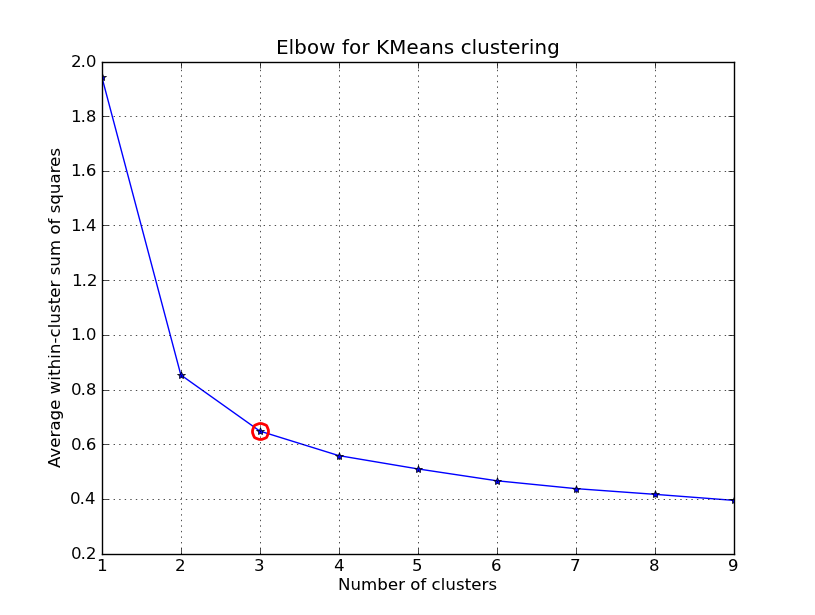
\includegraphics[scale=0.3]{images/elbow.png}    
    \end{column}
\end{columns}

\end{frame}

% ============================================== %

\begin{frame}{Критерий Silhouette}

Пусть дана кластеризация в $K$ кластеров, и объект $i$ попал в $C_k$

\vspace{1em}
\begin{itemize}
\item $a(i)$ -- среднее расстояние от $i$ объекта до объектов из $C_k$
\item $b(i) = min_{j \neq k} b_j(i)$,  где $b_j(i)$ -- среднее расстояние от $i$ объекта до объектов из $C_j$
\end{itemize}
\[
silhouette(i) = \frac{b(i) - a(i)}{\max(a(i), b(i))}
\]
Средний silhouette для всех точек из $\mathbf{X}$ является критерием качества кластеризации.

\end{frame}

% ============================================== %

\section{Иерархическая кластеризация}

% ============================================== %

\begin{frame}{Иерархическая кластеризация: идея метода}

{\bf Agglomerative}
\begin{enumerate}
\item начинаем с ситуации, когда каждый объект -- отдельный кластер
\item на каждом шаге совмещаем два наиболее близких кластера
\item останавливаемся, когда получаем требуемое количество или единственный кластер
\end{enumerate}

\vspace{1em}
Divisive
\begin{enumerate}
\item начинаем с ситуации, когда все объекты составляют один кластер
\item на каждом шаге разделяем два один из кластеров пополам
\item останавливаемся, когда получаем требуемое количество или $N$ кластеров
\end{enumerate}

\end{frame}

% ============================================== %

\begin{frame}{Дендрограмма}

\begin{center}
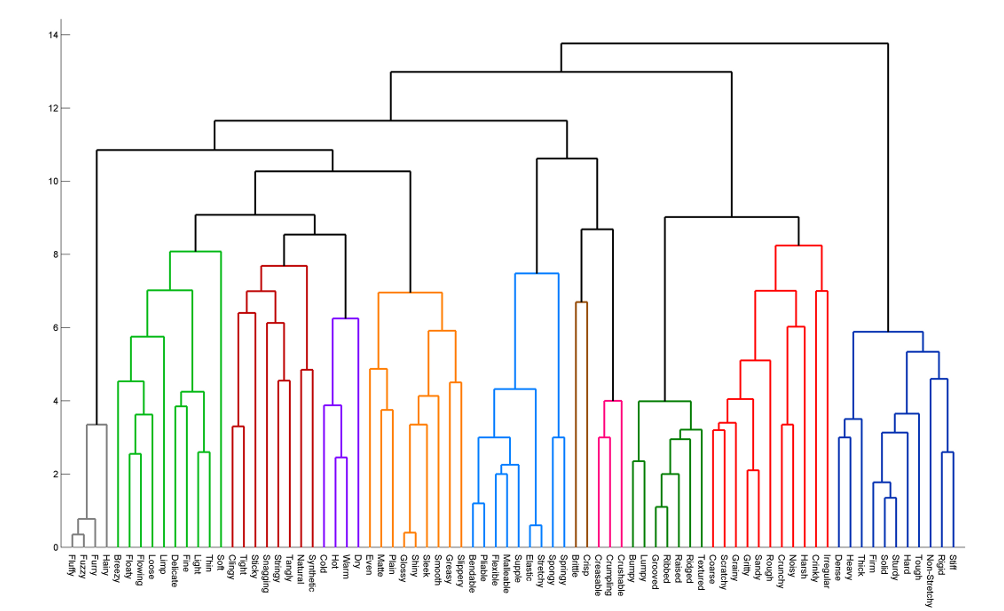
\includegraphics[scale=0.3]{images/dendro.png}
\end{center}

\end{frame}

% ============================================== %

\begin{frame}{Радиальная дендрограмма}

\begin{center}
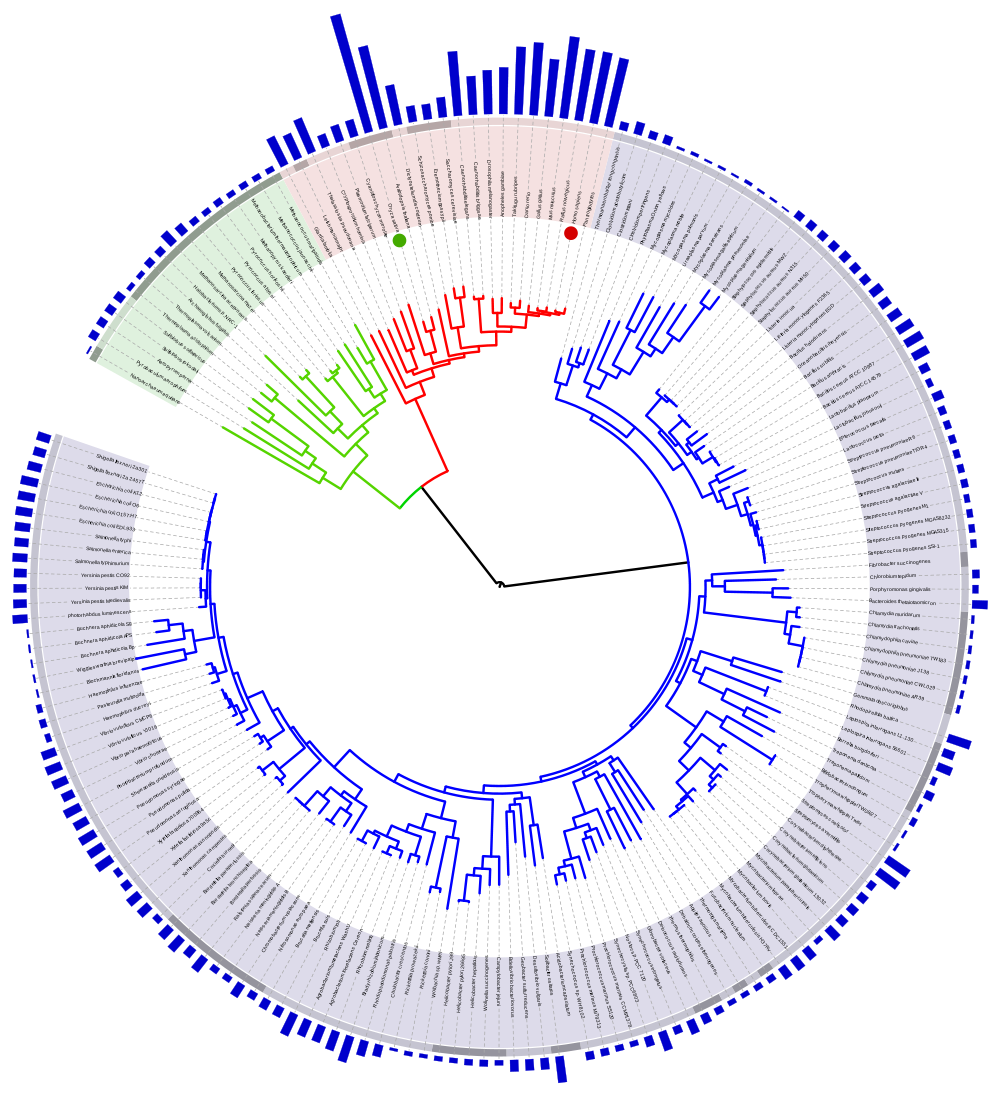
\includegraphics[scale=0.3]{images/radial.png}
\end{center}

\end{frame}

% ============================================== %

\begin{frame}{Агломеративный алгоритм}

\texttt{agglomerative($\mathbf{X}$, $K$):}

\texttt{\quad Инициализируем $C_i \leftarrow \mathbf{x}_i,\; C = N$}

\texttt{\quad do}

\texttt{\quad\quad Ищем ближайшие кластеры $C_i$ и $C_j$}

\texttt{\quad\quad Совмещаем ближайшие кластеры $C_i$ и $C_j$}

\texttt{\quad\quad $C = C - 1$}

\texttt{\quad until $C = K$ or $C = 1$}

\texttt{\quad return $C_1, \ldots, C_K$}

\vspace{1em}
Алгоритмическая сложность: $O(n^2 \log n)$

\end{frame}

% ============================================== %

\begin{frame}{Расстояние между кластерами}

\begin{itemize}
\item single-linkage
\[
d_{min}(C_i, C_j) = \min_{\mathbf{x} \in C_i, \mathbf{x}' \in C_j} \|\mathbf{x} -\mathbf{x}' \|
\]
\item complete-linkage
\[
d_{max}(C_i, C_j) = \max_{\mathbf{x} \in C_i, \mathbf{x}' \in C_j} \|\mathbf{x} -\mathbf{x}' \|
\]
\item average
\[
d_{avg}(C_i, C_j) = \frac{1}{n_i n_j}\sum_{\mathbf{x} \in C_i}\sum_{\mathbf{x}' \in C_j} \|\mathbf{x} -\mathbf{x}' \|
\]
\item mean
\[
d_{mean}(C_i, C_j) = \|\mathbf{m}_i -\mathbf{m}_j \|
\]
\end{itemize}

\end{frame}

% ============================================== %

\begin{frame}{Задача}

Кластеризовать данные иерархическим методом с использованием расстояний между кластерами $d_{min}$ и $d_{max}$
\begin{center}
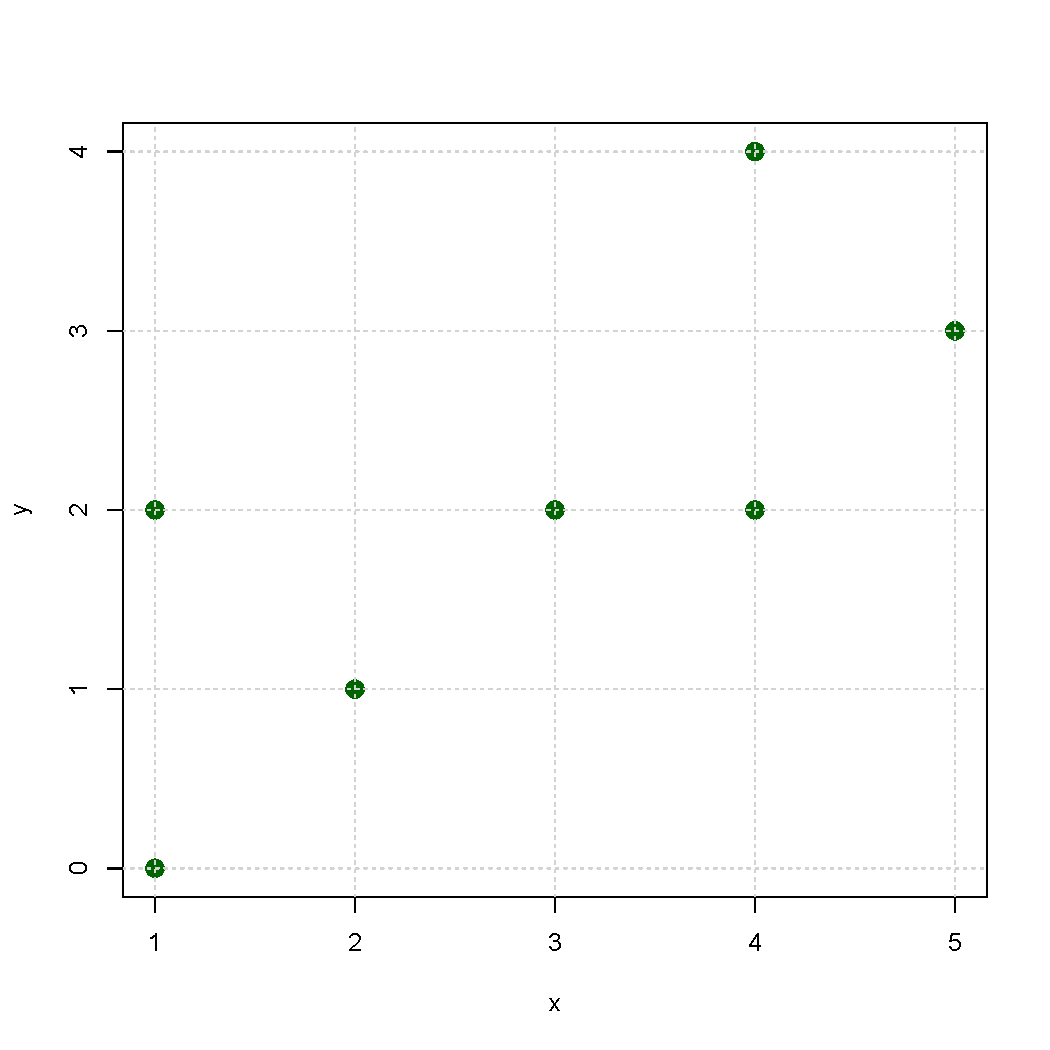
\includegraphics[scale=0.4]{images/problem.pdf}
\end{center}

\end{frame}

% ============================================== %

\begin{frame}{Stepwise-optimal HC}

Какой критерий мы оптимизируем?

\vspace{1em}
\texttt{swo($\mathbf{X}$, $K$):}

\texttt{\quad Инициализируем $C_i \leftarrow \mathbf{x}_i,\; C = N$}

\texttt{\quad do}

\texttt{\quad\quad Ищем $C_i$ и $C_j$, после совмещения которых }

\texttt{\quad\quad\;\; критерий оптимальности наиболее улучшится}

\texttt{\quad\quad Совмещаем ближайшие кластеры $C_i$ и $C_j$}

\texttt{\quad\quad $C = C - 1$}

\texttt{\quad until $C = K$ or $C = 1$}

\texttt{\quad return $C_1, \ldots, C_K$}

\vspace{1em}
$d_{max}$ обеспечивает наименьшее увеличение диаметра кластера \\
$d_e$ обеспечивает наименьшее увеличение квадратичного критерия
\[
d_e(C_i, C_j) = \sqrt{\frac{n_i n_j}{n_i + n_j}} \|\mathbf{m}_i -\mathbf{m}_j \|
\]

\end{frame}

% ============================================== %

\begin{frame}{Неэвклидовы пространства}

{\it Проблема. } Как измерить расстояние между кластерами, если невозможно определить центроид?

\vspace{1em}
{\it Идея. } В каждом из кластеров выбрать ``типичный'' пример -- clustroid.

\vspace{1em}
Минимизируем
\begin{itemize}
\item сумму расстояний до других объектов в кластере
\item сумму квадратов расстояний до других объектов в кластере
\item максимальное расстояние до других объектов в кластере
\end{itemize}

\end{frame}

% ============================================== %

\begin{frame}{Иерархическая кластеризация: итог}

\begin{itemize}
\item[+] Несферические кластеры
\item[+] Разнообразие критериев
\item[+] Любые $K$ из коробки
\item[---] Требует много ресурсов
\end{itemize}

\end{frame}

% ============================================== %

\section{DBSCAN}

% ============================================== %

\begin{frame}{DBSCAN: идея метода}

\begin{itemize}
\item Кластеризация, основанная на плотности объектов
\item Кластеры -- участки высокой плотности, разделенные участками низкой плотности
\end{itemize}

\begin{center}
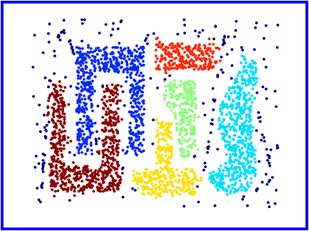
\includegraphics[scale=0.6]{images/dbscan.jpg}
\end{center}

\end{frame}

% ============================================== %

\begin{frame}{Определения}

\begin{block}{Плотность}
Количество объектов внутри сферы заданного радиуса $\varepsilon$
\end{block}

\begin{block}{Core-объект}
Объект $\mathbf{x}$ является core-объектом, если плотность вокруг него больше $min\_pts$
\end{block}

\begin{block}{Граничный-объект}
Объект $\mathbf{x}$ является граничным-объектом, если плотность вокруг него меньше $min\_pts$, но он находится рядом с core-объектом
\end{block}

\begin{block}{Шум}
Объект $\mathbf{x}$ является шумом, если он не является ни core-объектом, ни граничным объектом
\end{block}

\end{frame}

% ============================================== %

\begin{frame}{Виды объектов}

\begin{center}
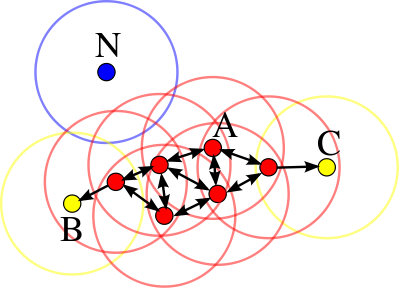
\includegraphics[scale=0.5]{images/points.png}
\end{center}

\end{frame}

% ============================================== %

\begin{frame}{DBSCAN 1}

\texttt{dbscan($\mathbf{X}$, $\varepsilon$, $min\_pts$):}

\texttt{\quad for не посещенные $P \in \mathbf{X}$:}

\texttt{\quad\quad помечаем $P$ как посещенный}

\texttt{\quad\quad $nbr = neigbors(P, \varepsilon)$}

\texttt{\quad\quad if $len(nbr) < min\_pts$:}

\texttt{\quad\quad\quad помечаем $P$ как шум}

\texttt{\quad\quad else:}

\texttt{\quad\quad\quad $C = create\_cluster()$}

\texttt{\quad\quad\quad $expand\_cluster(P, nbr, C, \varepsilon, min\_pts)$}

\texttt{\quad\quad\quad $yield\;C$}

\end{frame}

% ============================================== %

\begin{frame}{DBSCAN 2}

\texttt{expand\_cluster($P, nbr, C, \varepsilon, min\_pts$):}

\texttt{\quad добавляем $P$ в $C$}

\texttt{\quad for $P' \in nbr$:}

\texttt{\quad\quad if $P'$ не посещался:}

\texttt{\quad\quad\quad помечаем $P'$ как посещенный}

\texttt{\quad\quad\quad $nbr' = neighbors(P', \varepsilon)$}

\texttt{\quad\quad\quad if $len(nbr) \geq min\_pts$:}

\texttt{\quad\quad if $P'$ не принадлежит ни одному кластеру:}

\texttt{\quad\quad\quad добавляем $P'$ в $C$}

\vspace{1em}
Сложность: $O(n^2)$ или $O(n \log n)$ ($R^*Tree$) \\ 
Память: $O(n)$ или $O(n^2)$ 

\end{frame}

% ============================================== %

\begin{frame}{DBSCAN: итог}

\begin{columns}[C]
    \begin{column}{.6\textwidth} 
    \begin{itemize}
	\item[+] не требует $K$
	\item[+] кластеры произвольной формы
	\item[+] учитывает выбросы
	\item[---] Не вполне детерминированный
	\item[---] Не работает при разных плотностях кластеров
	\end{itemize}		    
    \end{column}
    \begin{column}{.4\textwidth}
    \vspace{1em}
    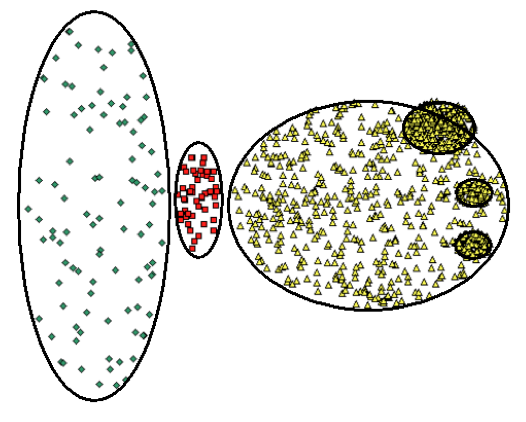
\includegraphics[scale=0.25]{images/dbprob.png}    
    \end{column}
\end{columns}

\end{frame}

% ============================================== %

\begin{frame}{Домашнее задание 2}

\begin{block}{Иерархическая кластеризация и DBCSAN}
Реализовать алгоритм иерархической кластеризации и DBSCAN и протестировать на данных задачи модуля
\end{block}

\vspace{1em}
Ключевые даты
\begin{itemize}
\item До 2014/05/03 00.00 выбрать ответственных
\item До 2014/05/10 00.00 предоставить решения (после -- половина очков)
\end{itemize}

\end{frame}

% ============================================== %

\begin{frame}{На сегодня}

\begin{enumerate}
\item Скачать ветку hier и запустить код для нескольких значений $n$
\item Реализовать метрики качества кластеризации
\begin{enumerate}
\item Средней квадрат отклонения от центра
\item Средний диаметр кластера
\item Silhouette
\end{enumerate}
Позволяют ли эти метрики верно выбрать число кластеров?
\end{enumerate}

\end{frame}

% ============================================== %

\end{document}